% Chapter Template

\chapter{Graph-Based Structural Output Learning} % Main chapter title
\label{Chapter3} % Change X to a consecutive number; for referencing this chapter elsewhere, use \ref{ChapterX}
\lhead{Chapter 3. \emph{Graph-Based Structural Output Learning}} % Change X to a consecutive number; this is for the header on each page - perhaps a shortened title



\rule{\textwidth}{0.4pt} \\[0.5cm]
\textit{``To learn without thinking is blindness; to think without learning is idleness. "}

\begin{flushright}
Confucius
\end{flushright}
\rule{\textwidth}{0.4pt} 

In chapter \ref{Chapter2}, modeling and inference of graphical models (mostly undirected ones) were explained. Meanwhile, until now, it is assumed that   
the parameters of potential functions are provided by an expert of a specific task. However, this is usually not the case in practice.      
Even though some empirical knowledge is available for specifying the parameters, it tends to be unreliable. 
A wiser strategy is to learn the parameters from some training data.      

This chapter focuses the learning of undirected graphical models, based on which structural data can subsequently be inferred.      
At first, in section \ref{sec:crf}, a special case of Markov network, \emph{conditional random field} (CRF), is introduced for the discriminative learning      
of structural-output. Its training issues and relation to \emph{max-margin Markov network} (M$^3$N) are studied as well.   
Second, in section \ref{sec:PSMC},  a new algorithm, \emph{persistent sequential Monte Carlo} (PSMC), 
is developed for learning general undirected graphical models.   

Another aspect in training graphical models is the learning of graph structures, which, however, is not covered in this thesis.    


%----------------------------------------------------------------------------------------
%	SECTION 1
%----------------------------------------------------------------------------------------
\section{Conditional Random Field}
\label{sec:crf}
In general supervised learning paradigm, there exist input and output: $\{\mathbf{x},\mathbf{y}\}$. The target is to learn a function       
$f:f(\mathbf{x})\rightarrow \mathbf{y}$ from a training dataset such that the estimated error of $\{f(\mathbf{x}),\mathbf{y}\}$ can be minimized.     
In classic machine learning, output is only a binary value or a single scalar, which corresponds to binary classification and regression respectively.      
However, with the increasingly higher data complexity in many areas, learning structural output are now more of interest.        

Markov networks, or Markov random fields (MRFs) can be used as a generative learning scheme for the learning task.    
A MRF is supposed to 
reconstruct the generative process by defining a joint probability of $\{\mathbf{x,y}\}: p(\mathbf{x,y})=p(\mathbf{x})p(\mathbf{y}|\mathbf{x})$. 
As for the prediction task, the conditional probability 
$p(\mathbf{y|x})=\frac{p(\mathbf{x,y})}{\sum_\mathbf{y} p(\mathbf{x,y})}$ can be derived, or more straightforwardly, 
$\mathbf{y}^*=\arg\max_{\mathbf{y}}p(\mathbf{y|x})=\arg\max_{\mathbf{y}}p(\mathbf{x,y})$ (\emph{e.g.} by using max-product algorithm). 
However, it was realised that for learning $f:\mathbf{x}\to\mathbf{y}$, the only desired
component is $p(\mathbf{y|x})$. It is wast to expend effort in modeling $p(\mathbf{x})$, which is not relevant anyway. Consequently, \emph{conditional random field} (CRF) was proposed \citep{CRF} as 
a discriminative model by learning only the conditional probability $p(\mathbf{y|x})$. One significant strength of CRFs in practice is that it can include arbitrarily complex features (\emph{e.g.} higher order dependencies) 
of $\mathbf{x}$, which is intractable in MRFs. According to empirical study in \citep{Kumar03,CRF}, CRFs outperform MRFs in many practical applications. 

At first, the definition of conditional random fields (CRFs) is given as \citep{CRF}: 
\begin{definition}
    Let $G=(V,E)$ be a graph ($V$ are vertices and $E$ are edges) such that $\mathbf{y}=\{y_v\}_{v\in V}$, so that $y$ is indexed by the vertices of $G$. Then $(\mathbf{x,y})$ is a 
        conditional random field in case, when conditioned on $\mathbf{x}$, the random variables $\{y_v\}_{v\in V}$ obey the Markov property with respect to 
    the graph $G$.   
\label{def:CRF}
\end{definition}
Assume that the joint conditional probability $p(\mathbf{y|x})$ is defined in an exponential form: 
\begin{equation}
    p(\mathbf{y|x})=\frac{\exp(\mathbf{w}^\top \boldsymbol{\phi}(\mathbf{x,y}))}{\mathbf{Z(w)}}
\end{equation}
where $\mathbf{x}\in\mathcal{X},\mathbf{y}\in\mathcal{Y}$, $\boldsymbol{\phi}(\mathbf{x,y})\in\mathbb{R}^K$ is a collection of $K$ predefined, task-specific potential functions  (or feature vectors)
$\boldsymbol{\phi}(\mathbf{x,y})=[\phi_1(\mathbf{x,y}),\cdots \phi_K(\mathbf{x,y})]^\top$, $\mathbf{w}\in\mathbb{R}^K$ is the parameter vector,  
$\mathbf{Z(w)}$ is the partition function for normalization $\mathbf{Z(w)}=\sum_{\mathbf{y}\in\mathcal{Y}} \exp(\mathbf{w}^\top \boldsymbol{\phi}(\mathbf{x,y}))$. 

As a probabilistic model, one CRF is usually 
learned via \emph{maximum likelihood estimation} (MLE) or \emph{maximum a posterior} (MAP) \citep{Kumar03,CRF,Accelerated_CRF}. 
Meanwhile, inspired by the margin notion which has been exploited in successful binary classifiers, \emph{e.g.} \emph{Support Vector Machine} (SVM),  
an alternative discriminative training scheme of CRFs is maximizing the margin between 
the $p(\mathbf{y|x})$ of the desired $\mathbf{y^*}$ and the best runner-up $\mathbf{y}^{**}$  in their $\log$ domains. The CRFs trained with this 
margin
are referred to as 
\emph{Max-Margin Markov Networks} (M$^3$Ns) \citep{Taskar03}. 
On the one hand, similarly to regular SVM, \emph{kernel tricks} can be used in the dual form of M$^3$N, in which way, the original inputs and/or outputs are implicitly mapped into a higher 
dimensional \emph{reproducing kernel Hilbert space} (RKHS) (\emph{e.g.} polynomial kernels used in \citep{Taskar03}).     
On the other hand, different from regular SVM, the \emph{quadratic programming} 
(QP) problem associated with M$^3$Ns (in both primal and dual form) has exponential number of constraints. 
Although it can be simplified by exploiting interesting properties within forest-structured outputs \citep{Taskar03},  
for highly connected graphs, the learning is intractable.      
Obviously, although CRF and  M$^3$Ns offer almost equivalent modeling capabilities for a given machine learning task, two rather different loss functions are 
employed in them. However, it will be revealed in next two subsections that MAP and max-margin learning schemes are, to large extent, related. 
%-----------------------------------
%	SUBSECTION 1
%-----------------------------------
\subsection{Maximum Likelihood Estimation}
\label{subsec:MLE}
Given a training dataset $\mathcal{D}=\{\mathbf{x}^{(i)},\mathbf{y}^{(i)}\}_{i=1}^M$, a CRF can be learned via maximum likelihood estimation (MLE):
\begin{equation}
    \begin{array}{rl}
        \mathbf{w}^* =& \arg\max_{\mathbf{w}} \frac{1}{M}\sum_{i=1}^M \log p(\mathbf{y}^{(i)}|\mathbf{x}^{(i)}) \\
                     =& \arg\max_{\mathbf{w}} \frac{1}{M}\sum_{i=1}^M \{\mathbf{w}^\top \boldsymbol{\phi}(\mathbf{x}^{(i)},\mathbf{y}^{(i)}) -\log \sum_{\mathbf{y}\in\mathcal{Y}} \exp(\mathbf{w}^\top \boldsymbol{\phi}(\mathbf{x}^{(i)},\mathbf{y}))\}
    \end{array}
    \label{equ:MLE}
\end{equation}
Meanwhile, usually, in order to enhance the generalization properties, a prior on $p(\mathbf{w})\propto \exp(-\frac{\mathbf{w}^2}{\sigma^2})$ is added in (\ref{equ:MLE}) to penalize the complexity of $\mathbf{w}$, which 
results in the maximum a posterior (MAP) solution:
\begin{equation}
    \begin{array}{rl}
        \mathbf{w}^* =& \arg\max_{\mathbf{w}}  -\frac{\mathbf{w}^2}{\sigma^2} +\frac{1}{M}\sum_{i=1}^M \{\mathbf{w}^\top \boldsymbol{\phi}(\mathbf{x}^{(i)},\mathbf{y}^{(i)}) -\log \sum_{\mathbf{y}\in\mathcal{Y}} \exp(\mathbf{w}^\top \boldsymbol{\phi}(\mathbf{x}^{(i)},\mathbf{y}))\}  \\ 
                     =& \arg\min_{\mathbf{w}} \frac{1}{2} ||\mathbf{w}||^2+  \frac{C}{M}\sum_{i=1}^M \mathcal{L}^{MAP}_i 
    \end{array}
    \label{equ:MAP}
\end{equation}
where $\mathcal{L}_i^{MAP}$ is the negative log-likelihood of the $i$th training instance:  
\begin{equation}
    \mathcal{L}^{MAP}_i=\log \sum_{\mathbf{y}\in\mathcal{Y}} \exp(\mathbf{w}^\top \boldsymbol{\phi}(\mathbf{x}^{(i)},\mathbf{y}))-\mathbf{w}^\top \boldsymbol{\phi}(\mathbf{x}^{(i)},\mathbf{y}^{(i)})
    \label{equ:MAP_loss}
\end{equation}
and $C=\frac{\sigma^2}{2}$ is a trade-off parameter to balance the regularization term $\frac{1}{2} ||\mathbf{w}||^2$ and average loss $\frac{1}{M}\sum_{i=1}^M \mathcal{L}^{MAP}_i$. A good property 
of (\ref{equ:MAP}) is that it is convex with respect to $\mathbf{w}$. 
\begin{proposition}
    The objective function of maximum a posterior in learning CRFs is convex.
\label{pro:MAP_convex}
\end{proposition}

\begin{proof}
    The second order derivative of $\log \sum_{\mathbf{y}} \exp(\mathbf{w}^\top \boldsymbol{\phi}(\mathbf{x}^{(i)},\mathbf{y}))$ with respect to 
    $\mathbf{w}$ is:
    \begin{equation}
    \frac{d^2 \log \sum_{\mathbf{y}} \exp(\mathbf{w}^\top \boldsymbol{\phi}(\mathbf{x}^{(i)},\mathbf{y}))}{d \mathbf{w}^2}=\mathbf{Cov}_{p(\mathbf{y}|\mathbf{x}^{(i)};\mathbf{w})}\boldsymbol{\phi}(\mathbf{x}^{(i)},\mathbf{y})
    \end{equation}
    where $\mathbf{Cov}_{p(\boldsymbol{\rho})}f(\boldsymbol{\rho})$ denotes the covariance of $f(\boldsymbol{\rho})$ under the probability $p(\boldsymbol{\rho})$. 
    Since the covariance function is always positive semidefinite, $\log \sum_{\mathbf{y}} \exp(\mathbf{w}^\top \boldsymbol{\phi}(\mathbf{x}^{(i)},\mathbf{y}))$ is convex. In addition, 
    $-\mathbf{w}^\top \boldsymbol{\phi}(\mathbf{x}^{(i)},\mathbf{y}^{(i)})$ is linear (thus also convex), and $\frac{1}{2} ||\mathbf{w}||^2$ is convex. Therefore, 
    (\ref{equ:MAP}) (the sum of convex components) is convex.  
\end{proof}
Because of the convexity of the objective function, any local minimum is also global minimum, and gradient descent can be employed to find the unique solution 
$\mathbf{w}^*$ with the negative gradient computed as: 
\begin{equation}
    \Delta \mathbf{w}_t=\frac{C}{M}\sum_{i=1}^M(\boldsymbol{\phi}(\mathbf{x}^{(i)},\mathbf{y}^{(i)})-\mathbb{E}_{p(\mathbf{y}|\mathbf{x}^{(i)};\mathbf{w}_t)} \boldsymbol{\phi}(\mathbf{x}^{(i)},\mathbf{y}))-\mathbf{w}_t 
\label{equ:gradient_MAP}
\end{equation}
where $\mathbb{E}_{p(\boldsymbol{\rho})}f(\boldsymbol{\rho})$ is the expectation of $f(\boldsymbol{\rho})$ under the probability $p(\boldsymbol{\rho})$.
The difficulty of computing (\ref{equ:gradient_MAP}) is the expectation term because its complexity grows exponentially. For example, in multi-label 
learning case introduced in section \ref{sec:crf}, $|\mathcal{Y}|=2^L$. 
Therefore, when $|\mathcal{Y}|$ is relatively large in practice, enumerating all possible $\mathbf{y}$ is impossible. 
In addition, as studied in section \ref{sec:inference}, exact inference within loopy graphs is intractable, therefore some approximations were used for learning: 
\emph{e.g.} \emph{mean field} (MF), \emph{loopy belief propagation} (LBP) or \emph{pseudo likelihood} (PL) \citep{LBP, Kumar03,CRF,Accelerated_CRF}.  



\subsection{Max-Margin Markov Network}
\label{subsec:MMMN}
The max-margin principle used in binary classifier, \emph{e.g.} Support Vector Machine (SVM), has been proven theoretically and empirically \citep{Vapnik} superior to others.        
The margin notion was generalized to learn structured outputs in \citep{Taskar03} and structural SVM \citep{StructSVM}. More concretely, they proposed to learn CRFs by maximizing the margin 
between the $p(\mathbf{y|x})$ of the desired $\mathbf{y^*}$ and the best runner-up $\mathbf{y}^{**}$ in log domain. The CRFs trained with maximum margin are referred to as 
max-margin Markov networks (M$^3$Ns) \citep{Taskar03}.  The objective function of a M$^3$N can be written out as: 
\begin{equation}
    \begin{array}{rl}
        & \arg\min_{\mathbf{w},\xi_{i:i\in[1,M]}}  \frac{1}{2} ||\mathbf{w}||^2 +\frac{C}{M} \sum_{i=1}^M \xi_i \\
   s.t. &\forall i, \forall y\in\mathcal{Y}/\mathbf{y}^{(i)}: \xi_i\geq0, \mathbf{w}^\top (\boldsymbol{\phi}(\mathbf{x}^{(i)},\mathbf{y}^{(i)})-\boldsymbol{\phi} 
        (\mathbf{x}^{(i)},\mathbf{y}))\geq 1-\frac{\xi_i}{d(\mathbf{y}^{(i)},\mathbf{y})}
    \end{array}
    \label{equ:MMMN}
\end{equation}
where $\xi_i$ are slack variables for the relaxation of 
max-margin, and $d(\mathbf{y}^{(i)},\mathbf{y})\geq0$ is a measure of dissimilarity between $\mathbf{y}^{(i)}$ and $\mathbf{y}$ 
(\emph{e.g.} hamming distance used in the multilable learning case). The term $\frac{\xi_i}{d(\mathbf{y}^{(i)},\mathbf{y})}$ is to rescale 
slack variables by the dissimilarities between corresponding $\mathbf{y}^{(i)}$ and others. 
Obviously, (\ref{equ:MMMN}) is a quadratic programming (QP)  problem with exponential number of 
constraints. Similarly to SVM, (\ref{equ:MMMN}) can be converted to its dual form, of which some interesting properties can be exploited 
to simplify the computation 
for forest-structured outputs (\emph{i.e.} singly-connected graphs). However, for highly-connected graphs, the exact learning of M$^3$Ns is intractable.  
An advantage of the dual form of M$^3$N is that it enables the use of \emph{kernel methods}, which can implicitly project 
$\boldsymbol{\phi}(\mathbf{x},\mathbf{y})$ to 
a higher dimensional Hilbert feature space. Defining $\boldsymbol{\phi}(\mathbf{x},\mathbf{y})$  with kernel methods was more exploited in Structural SVM \citep{StructSVM} (see subsection \ref{subsec:SSVM}). 
Usually quadratic or cubic kernels are used and yield promising results \citep{Taskar03}. 
Correspondingly, 
explicitly feature map of $\boldsymbol{\phi}(\mathbf{x},\mathbf{y})$  can be constructed via two-degree and three-degree polynomials in the primal form of M$^3$Ns.  

The second constraint in (\ref{equ:MMMN}) can be written in a more compact form: 
$\max_{\mathbf{y}\in\mathcal{Y}} \{d(\mathbf{y}^{(i)},\mathbf{y})-{\mathbf{w}^\top} (\boldsymbol{\phi}(\mathbf{x}^{(i)},\mathbf{y}^{(i)})-\boldsymbol{\phi} 
        (\mathbf{x}^{(i)},\mathbf{y})) d(\mathbf{y}^{(i)},\mathbf{y}\}\leq \xi_i$. 
In addition, $\mathbf{w}$ can be rescaled $\mathbf{w}\gets \mathbf{w}d(\mathbf{y}^{(i)},\mathbf{y})$. 
Then, instead of rescaling slack variables, one can rescale margin to be the same level as 
$d(\mathbf{y}^{(i)},\mathbf{y})$.  
Therefore, (\ref{equ:MMMN}) can be reformulated in a similar form as (\ref{equ:MAP}):
\begin{equation}
        \mathbf{w}^* = \arg\min_{\mathbf{w}} \frac{1}{2} ||\mathbf{w}||^2+ \frac{C}{M}\sum_{i=1}^M \mathcal{L}^{Margin}_i 
    \label{equ:MMMN_compact}
\end{equation}
where 
\begin{equation} 
    \mathcal{L}^{Margin}_i=\max_{\mathbf{y}\in\mathcal{Y}} \{d(\mathbf{y}^{(i)},\mathbf{y})+ \mathbf{w}^\top\boldsymbol{\phi} 
        (\mathbf{x}^{(i)},\mathbf{y})\} -\mathbf{w}^\top\boldsymbol{\phi}(\mathbf{x}^{(i)},\mathbf{y}^{(i)})
\label{equ:MMMN_loss}
\end{equation}



Based on the introduction of CRFs and M$^3$N above, a unified objective function for structured output learning  can be written out as:  
\begin{equation} 
        \mathbf{w}^* = \arg\min_{\mathbf{w}} \frac{1}{2} ||\mathbf{w}||^2+  \frac{C}{M}\sum_{i=1}^M \mathcal{L}_i 
    \label{equ:unify}
\end{equation} 
where $\mathcal{L}_i$ denote loss functions, which correspond to $\mathcal{L}^{MAP}_i$  employed in MAP and $\mathcal{L}^{Margin}_i$ used 
in M$^3$N respectively.      
Although, at a fist glance, two loss functions look rather different, they are de facto closely related. This section will provide deep insights  
into the behaviours of two loss functions.  
%within which the connections and differences between them can be more clearly exposed. 
At first, the feature vector in CRFs can be augmented by adding an extra component $d(\mathbf{y}^{(i)},\mathbf{y})$:  
$\bar{\boldsymbol{\phi}}(\mathbf{x}^{(i)},\mathbf{y})^\top=[\boldsymbol{\phi}(\mathbf{x}^{(i)},\mathbf{y})^\top,d(\mathbf{y}^{(i)},\mathbf{y})]$, 
and $\mathbf{w}$ is extended with a constant 1: $\bar{\mathbf{w}}^\top=[\mathbf{w}^\top, 1]$. Then the modified CRF distribution is:
\begin{equation}
    \bar{p}(\mathbf{y}|\mathbf{x})=\frac{\exp(\bar{\mathbf{w}}^\top \bar{\boldsymbol{\phi}}(\mathbf{x,y}))}{\mathbf{Z(\bar{w})}}
\end{equation}
Since $d(\mathbf{y}^{(i)},\mathbf{y}^{(i)})=0$, the resulting $\bar{\mathcal{L}}^{MAP}_i$ is:
\begin{equation}
    \begin{array}{cl}
        \bar{\mathcal{L}}^{MAP}_i      =&\log \sum_{\mathbf{y}\in\mathcal{Y}} \exp(\bar{\mathbf{w}}^\top \bar{\boldsymbol{\phi}}(\mathbf{x}^{(i)},\mathbf{y}))-\bar{\mathbf{w}}^\top \bar{\boldsymbol{\phi}}(\mathbf{x}^{(i)},\mathbf{y}^{(i)}) \\ 
                                       =&\log \sum_{\mathbf{y}\in\mathcal{Y}} \exp\big(\mathbf{w}^\top \boldsymbol{\phi}(\mathbf{x}^{(i)},\mathbf{y})+d(\mathbf{y}^{(i)},\mathbf{y})\big) -\mathbf{w}^\top \boldsymbol{\phi}(\mathbf{x}^{(i)},\mathbf{y}^{(i)}) 
\end{array}
    \label{equ:new_MAP_loss}
\end{equation}
$\bar{\mathcal{L}}^{MAP}_i$ was also named as ``softmax-margin" by \cite{SoftMax}. It can be easily proved that $\bar{\mathcal{L}}^{MAP}_i$ is convex by following a similar proof in {Proposition \ref{pro:MAP_convex}}
(note that $d(\mathbf{y}^{(i)},\mathbf{y})$ is independent of $\mathbf{w}$). It can be seen in (\ref{equ:MMMN_loss}) and (\ref{equ:new_MAP_loss}) that two loss functions share a similar form. The only 
difference between them is that the \emph{max} function is used in (\ref{equ:MMMN_loss}) while the \emph{log-sum-exp} function is used (\ref{equ:new_MAP_loss}) (the first term). 

Here, \textbf{the first connection} between $\mathcal{L}^{Margin}_i$ and $\bar{\mathcal{L}}^{MAP}_i$ is claimed:   
\begin{equation}
    \mathcal{L}^{Margin}_i \leq \bar{\mathcal{L}}^{MAP}_i\leq\mathcal{L}^{Margin}_i+\log |\mathcal{Y}|
    \label{equ:bound}
\end{equation}
\emph{i.e.} $\mathcal{L}^{Margin}_i$  
is a lower bound of $\mathcal{L}^{MAP}_i$ and specifies a upper bound of $\mathcal{L}^{MAP}_i$ by $\mathcal{L}^{Margin}_i+\log |\mathcal{Y}|$. For notation simplicity, $\pi_n$ is used to represent  
$\mathbf{w}^\top \boldsymbol{\phi}(\mathbf{x}^{(i)},\mathbf{y}_n)+d(\mathbf{y}^{(i)},\mathbf{y}_n)$, $\forall \mathbf{y}_n\in\mathcal{Y}$, and $|\mathcal{Y}|=N$. 
\begin{proposition}
    Given a set $\{\pi_n\in\mathbb{R}\}_{n=1}^N, \max\{\pi_n\}_{n=1}^N \leq \log\sum_{n=1}^N e^{\pi_n}\leq \max\{\pi_n\}_{n=1}^N+\log N$. 
\label{pro:bound}
\end{proposition}

\begin{proof}
    Since $\max\{e^{\pi_n}\}_{n=1}^N \leq \sum_{n=1}^N e^{\pi_n}\leq  N \max\{e^{\pi_n}\}_{n=1}^N$, 
    by taking the logarithm of above inequalities, it is obvious that    
    $\max\{\pi_n\}_{n=1}^N \leq \log\sum_{n=1}^N e^{\pi_n}\leq \max\{\pi_n\}_{n=1}^N\\+\log N$. 
    \label{proof:bound}
\end{proof}

\textbf{The second connection} between $\mathcal{L}^{Margin}_i$ and $\bar{\mathcal{L}}^{MAP}_i$ is:  
given two solutions of $\mathcal{L}_i^{Margin}$, $\mathbf{w}_1$  and $\mathbf{w}_2$.   
\begin{equation}
    \begin{array}{rcl}
        \text{when} & &\max_{\mathbf{y}\in\mathcal{Y}}\bar{p}(\mathbf{y}|\mathbf{x}^{(i)};\mathbf{w}_1)> \max_{\mathbf{y}\in\mathcal{Y}}\bar{p}(\mathbf{y}|\mathbf{x}^{(i)};\mathbf{w}_2),\\ 
                    & &\bar{\mathcal{L}}_i^{MAP}(\mathbf{w}_1)-\mathcal{L}_i^{Margin}(\mathbf{w}_1) < \bar{\mathcal{L}}_i^{MAP}(\mathbf{w}_2)-\mathcal{L}_i^{Margin}(\mathbf{w}_2) 
    \end{array}
\label{equ:monotomic}
\end{equation}
\emph{i.e.} the gap $\bar{\mathcal{L}}_i^{MAP}(\mathbf{w})-\mathcal{L}_i^{Margin}(\mathbf{w})$ monotonically decreases with respect to $\max_{\mathbf{y}\in\mathcal{Y}}\bar{p}(\mathbf{y}|\mathbf{x}^{(i)};\mathbf{w})$. 
Likewise, let $\pi_n$ represent  
$\mathbf{w}_1^\top \boldsymbol{\phi}(\mathbf{x}^{(i)},\mathbf{y}_n)+d(\mathbf{y}^{(i)},\mathbf{y}_n)$ and $\tau_n$ represent 
$\mathbf{w}_2^\top \boldsymbol{\phi}(\mathbf{x}^{(i)},\mathbf{y}_n)+d(\mathbf{y}^{(i)},\mathbf{y}_n)$, $\forall \mathbf{y}_n\in\mathcal{Y}$. 
\begin{proposition}
    Given two sets of the same size $N$, $\{\pi_n\in\mathbb{R}\}_{n=1}^N$ and $\{\tau_n\in\mathbb{R}\}_{n=1}^N$. In addition, $p_t^\pi=\frac{\exp(\pi_t)}{\sum_{n=1}^N\exp(\pi_n)}$ 
    and $p_t^\tau=\frac{\exp(\tau_t)}{\sum_{n=1}^N\exp(\tau_n)}$. Then $\log\sum_{n=1}^N\\ \exp{\pi_n}-\max\{\pi_n\}_{n=1}^N< \log\sum_{n=1}^N \exp{\tau_n}-\max\{\tau_n\}_{n=1}^N$ when 
    $\max\{ p_t^\pi\}>\max\{ p_t^\tau\}$.   
\label{pro:monotomic}
\end{proposition}
\begin{proof}
    $\alpha=\log \sum_{n=1}^M \exp{\pi_n}-\max\{\pi_n\}_{n=1}^N=-\log (\max\{p^\pi_n\})$, $\beta=\log \sum_{n=1}^N\\\exp{\tau_n}-\max\{\tau_n\}_{n=1}^N=-\log (\max\{p^\tau_n\})$. So $\alpha-\beta=
    \log \frac{\max \{p^\tau_n\}}{\max \{p^\pi_n\}}$, and $\alpha-\beta<0 \Leftrightarrow \max \{p^\pi_n\}>\max \{p^\tau_n\}$.     
\end{proof}


\textbf{The third connection} between $\mathcal{L}^{Margin}_i$ and $\bar{\mathcal{L}}^{MAP}_i$ is: 
\begin{equation}
    \text{when} \max_{\mathbf{y}\in\mathcal{Y}}\{\bar{p}(\mathbf{y}|\mathbf{x}^{(i)})\}= 1, \quad \bar{\mathcal{L}}_i^{MAP}=\mathcal{L}^{Margin}_i 
    \label{equ:tight}
\end{equation}
\emph{i.e.} $\bar{\mathcal{L}}_i^{MAP}$ and $\mathcal{L}^{Margin}_i$ are identical when the conditional distribution $\bar{p}(\mathbf{y}|\mathbf{x}^{(i)})$ is a Dirac impulse concentrated on 
the outputs with the largest confidence score. 
\begin{proposition}
    Given a set $\{\pi_n\in\mathbb{R}\}_{n=1}^N$, and $p_t^\pi=\frac{\exp(\pi_t)}{\sum_{n=1}^N\exp(\pi_n)}$. Then $\log\sum_{n=1}^N\\\exp\pi_n-\max\{\pi_n\}=0$ when $\max\{p^\pi_n\}=1$.     
    \label{pro:bound}
\end{proposition}

\begin{proof}  
    $\log\sum_{n=1}^N\exp\pi_n-\max\{\pi_n\}=-\log (\max\{p^\pi_n\})$, so $\log\sum_{n=1}^N 
    \exp\pi_n-\max\{\pi_n\}=0$ when $\max\{p^\pi_n\}=1$.    
    \label{proof:bound}
\end{proof}

At last, \textbf{the forth connection} between $\mathcal{L}^{Margin}_i$ and $\bar{\mathcal{L}}^{MAP}_i$ is: 
\begin{equation}
    \text{when} \forall \mathbf{y}_n,\mathbf{y}_q\in\mathcal{Y}, \bar{p}(\mathbf{y}_n|\mathbf{x}^{(i)})= \bar{p}(\mathbf{y}_q|\mathbf{x}^{(i)}), \quad \bar{\mathcal{L}}_i^{MAP}=\mathcal{L}^{Margin}_i+\log|\mathcal{Y}|  
    \label{equ:upper_bound}
\end{equation}
\emph{i.e.} $\bar{\mathcal{L}}_i^{MAP}=\mathcal{L}^{Margin}_i+\log|\mathcal{Y}|$ when the conditional distribution $\bar{p}(\mathbf{y}|\mathbf{x}^{(i)})$ holds the largest entropy.    
\begin{proposition}
    Given a set $\{\pi_n\in\mathbb{R}\}_{n=1}^N$, and $p_t^\pi=\frac{\exp(\pi_t)}{\sum_{n=1}^N\exp(\pi_n)}$. Then 
    $\log\sum_{n=1}^N\\ \exp\pi_n=\max\{\pi_n\}+\log N$ when $\pi_n=\pi_q, \forall n,q \in [1,N]$.  
    \label{pro:up_bound}
\end{proposition}
\begin{proof}  
    $\log\sum_{n=1}^N\exp\pi_n-\max\{\pi_n\}=\log\frac{N\exp(\max\{\pi_n\})}{\exp(\max\{\pi_n\})}=\log N$.    
    \label{proof:up_bound}
\end{proof}
 
Combining four connections between $\bar{\mathcal{L}}^{MAP}_i$ and $\mathcal{L}^{Margin}_i$, it can be somehow concluded that the gap between $\bar{\mathcal{L}}^{MAP}_i$ and $\mathcal{L}^{Margin}_i$ ($\bar{\mathcal{L}}^{MAP}_i-\mathcal{L}^{Margin}_i$) is correlated 
with the entropy (or smoothness) of the 
conditional distributions exhibited in CRFs. The minimum gap is 0 when CRFs are collections of Dirac impulses, while the maximum gap is $\log|\mathcal{Y}|$ when conditional distributions 
are uniform.  
\cite{MaxEnt} and \cite{Norm_Partition} discovered roughly similar connections by increasing the sharpness of CRFs' output distributions with a tunable inverse temperature parameter, and a norm-defining 
parameter respectively. Four connections can be summarized by listing three extreme circumstances as follows: \\ \\
\begin{tabular}{m{15cm}}
      \Xhline{3\arrayrulewidth} \\ 
      when $\bar p(\mathbf{y}^{(i)}|\mathbf{x}^{(i)})\to 1$: $\mathbf{w}^\top \boldsymbol\phi(\mathbf{x}^{(i)},\mathbf{y}^{(i)})\gg \mathbf{w}^\top \boldsymbol\phi(\mathbf{x}^{(i)},\mathbf{y}^\prime)
        +d(\mathbf{y}^{(i)},\mathbf{y}^\prime), 
        \forall \mathbf{y}^\prime\in\mathcal{Y}/\mathbf{y}^{(i)}$, then $\mathcal{L}_i^{Margin}=0$, and $\mathcal{L}_i^{MAP}\to 0$;  \\ \\
      when $\exists \mathbf{y}^\prime\in\mathcal{Y}/\mathbf{y}^{(i)}, p(\mathbf{y}^\prime|\mathbf{x}^{(i)})\to 1$: $\mathbf{w}^\top \boldsymbol\phi(\mathbf{x}^{(i)},\mathbf{y}^{(i)})\ll \mathbf{w}^\top \boldsymbol\phi(\mathbf{x}^{(i)},\mathbf{y}^\prime)
        +d(\mathbf{y}^{(i)},\mathbf{y}^\prime)$, then $\mathcal{L}_i^{MAP}\to \infty$, and $\mathcal{L}_i^{MAP}-\mathcal{L}_i^{Margin}\to 0$ \\
      \Xhline{3\arrayrulewidth} \\
when $\forall \mathbf{y}_n, \mathbf{y}_q\in\mathcal{Y}, \bar p(\mathbf{y}_n|\mathbf{x}^{(i)})=\bar p(\mathbf{y}_q|\mathbf{x}^{(i)})$: $\mathbf{w}^\top \boldsymbol\phi(\mathbf{x}^{(i)},
        \mathbf{y}^{(i)})=\mathbf{w}^\top \boldsymbol\phi(\mathbf{x}^{(i)},\mathbf{y}^\prime)
        +d(\mathbf{y}^{(i)},\mathbf{y}^\prime), 
        \forall \mathbf{y}^\prime\in\mathcal{Y}/\mathbf{y}^{(i)}$, then $\mathcal{L}_i^{Margin}=0$, and $\mathcal{L}_i^{MAP}=\log |\mathcal{Y}|$;  \\ \\
\Xhline{3\arrayrulewidth}
\end{tabular}
\newline 
\newline 
These three cases do not look so interesting because they are unrealistic in practice.
However, these analysis will be of help for understanding the regularization in the next section.   


\subsection{Regularization as Maximum Entropy}
This subsection will study the effect of l2-norm 
regularization in MAP and max-margin learning respectively, and provide an alternative interpretation of its role: \emph{maximum entropy}.

\subsubsection{Maximum Entropy while Maximizing Margin}
At first, conditional distributions $\bar p(\mathbf{y}|\mathbf{x}^{(i)})$ learned 
with $\mathcal{L}_i^{Margin}$ are considered. As discussed in the previous section, when $\mathcal{L}_i^{Margin}$ is minimized to 0,       
$\bar p(\mathbf{y}|\mathbf{x}^{(i)})$ can still exhibit different shapes, which correspondingly will lead to different landscapes of 
$\mathbf{w}^\top\boldsymbol{\phi}(\mathbf{x}^{(i)},\mathbf{y})$. For example, in Figure \ref{fig:M3N_outputs_both} two different $\bar p(\mathbf{y}|\mathbf{x}^{(i)})$ and 
corresponding  $\mathbf{w}^\top\boldsymbol{\phi}(\mathbf{x}^{(i)},\mathbf{y})$ are presented (for simplicity $|\mathcal{Y}|=5$ is used).                
In Figure \ref{fig:M3N_outputs}, $p(\mathbf{y}^{(i)}|\mathbf{x}^{(i)})>p(\mathbf{y}^{\prime}|\mathbf{x}^{(i)}),\forall \mathbf{y}^\prime\in \mathcal{Y}/\mathbf{y}^{(i)}$, however, entropy 
is small because $p(\mathbf{y}^{(i)}|\mathbf{x}^{(i)})$ exceeds different $p(\mathbf{y}^{\prime}|\mathbf{x}^{(i)})$ to different degrees. In Figure \ref{fig:M3N_outputs_smooth},    
$p(\mathbf{y}^{(i)}|\mathbf{x}^{(i)})=p(\mathbf{y}^{\prime}|\mathbf{x}^{(i)}),\forall \mathbf{y}^\prime\in \mathcal{Y}/\mathbf{y}^{(i)}$ and thus entropy is maximized.     
Assume that there are two solutions of a M$^3$N with 0 loss, $\mathbf{w}_1$ and $\mathbf{w}_2$, which yield $\bar p(\mathbf{y}|\mathbf{x}^{(i)})$ as in Figure (\ref{fig:M3N_outputs}) and 
Figure (\ref{fig:M3N_outputs_smooth}) respectively. Then a first natural question to ask is: which one should be pursued?    
Usually the max-entropy case (Figure \ref{fig:M3N_outputs_smooth}) is preferred, and this preference can be explained from two perspectives: 
\begin{enumerate}
        \item The first motivation is   
            the well-known \emph{principle of maximum entropy} \citep{max_entropy_NLP}: once the loss function $\mathcal{L}_i^{Margin}$ is minimized, it is unsafer to impose any more assumptions on $\bar p(\mathbf{y}|\mathbf{x}^{(i)})$ without 
any extra information, \emph{i.e.} uniform $\bar p(\mathbf{y}|\mathbf{x}^{(i)})$  is more desirable.
        \item Secondly, as we can see in the lower part of Figure 
\ref{fig:M3N_outputs_smooth}, when $\bar p(\mathbf{y}|\mathbf{x}^{(i)})$ is uniform, the set 
$\{\mathbf{w}^{\top}(\boldsymbol{\phi}(\mathbf{x}^{(i)},\mathbf{y}^{(i)})-\boldsymbol{\phi}(\mathbf{x}^{(i)},\mathbf{y}^\prime)),\mathbf{y}^\prime\in \mathcal{Y}/\mathbf{y}^{(i)}\}$ is well 
aligned with the set  $\{d(\mathbf{y}^{(i)},\mathbf{y}^\prime)\}$. For all 
$i\in[1,M]$, when $\boldsymbol{\phi}(\mathbf{x}^{(i)},\mathbf{y}_n)-\boldsymbol{\phi}(\mathbf{x}^{(i)},\mathbf{y}_q)$ is projected on to $\mathbf{w}$, it equals 
to $d(\mathbf{y}_n,\mathbf{y}_q)$. Therefore, when $|\mathcal{D}|$ is relatively large, it can be intuitively envisioned that the gap between two points in $p(\mathbf{\mathbf{y}|\mathbf{x}})$ is 
consistent for all $\mathbf{x}\in\mathcal{X}$, which is better than a collection of distorted conditional distributions ($\{p(\mathbf{y}|\mathbf{x}^{(i)})\}_{i=1}^M$. This property is somehow 
in line with the findings in \cite{input-output_alignment}, where maximum alignment between inputs and outputs is pursued.      
\end{enumerate}
In M$^3$Ns, l2-norm regularization is usually considered as a penalty on the complexity of $\mathbf{w}$. Meanwhile, when $\mathcal{L}_0^{Margin}=0$,  
$\mathbf{w}^{\top}(\boldsymbol{\phi}(\mathbf{x}^{(i)},\mathbf{y}^{(i)})-\boldsymbol{\phi}(\mathbf{x}^{(i)},\mathbf{y}^\prime))$ will be closer to $d(\mathbf{y}^{(i)},\mathbf{y}^\prime)$ 
if $||\mathbf{w}||$ gets smaller. Therefore, the role of l2-norm regularization in M$^3$N can be re-interpreted as entropy maximization.       
\begin{figure}[t]
    \centering
    \subfigure[]{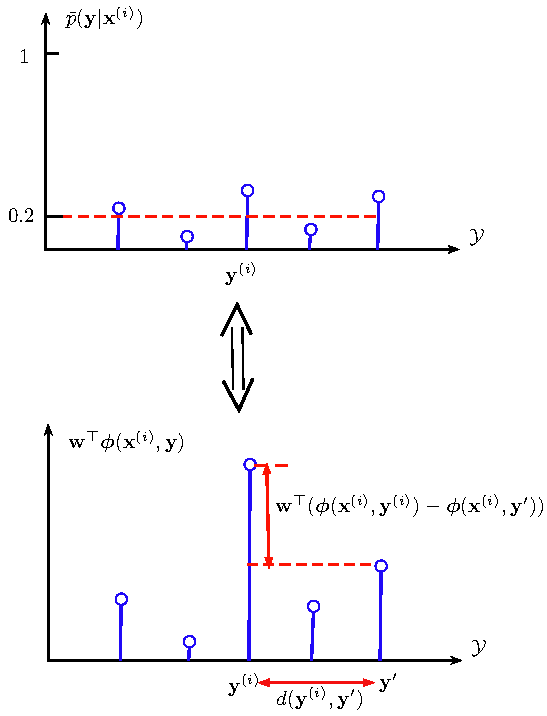
\includegraphics[width=0.49\textwidth]{./Figures/M3N_outputs.pdf}\label{fig:M3N_outputs}}
    \subfigure[]{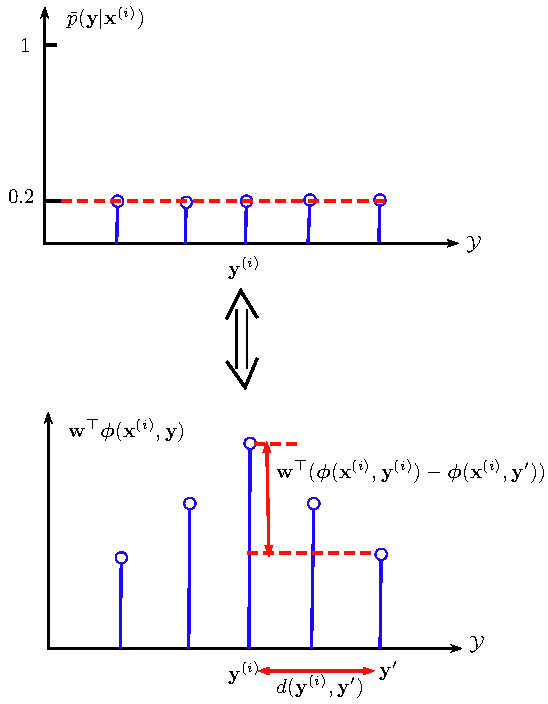
\includegraphics[width=0.49\textwidth]{./Figures/M3N_outputs_smooth.pdf}\label{fig:M3N_outputs_smooth}}
    \caption{Two possible cases  of $p(\mathbf{y}|\mathbf{x}^{(i)})$ and corresponding $\mathbf{w}^\top\boldsymbol{\phi}(\mathbf{x}^{(i)},\mathbf{y})$, when $\mathcal{L}^{Margin}$ is minimized. } 
    \label{fig:M3N_outputs_both}
\end{figure}



\subsubsection{Maximum Entropy within MAP Learning}
For simplicity, at first it is assumed that there exists only one training instance $\{\zeta,t\}$ in $\mathcal{D}$.  
Since $\bar{\mathcal{L}}^{MAP}_\zeta$ is convex, the gradient of minimum point $\mathbf{w}^*$ is 0: 
\begin{equation}
    \left.\frac{d \bar{\mathcal{L}}^{MAP}_\zeta}{d \mathbf{w}}\right|_{\mathbf{w}^*}=\boldsymbol{\phi}(\zeta, t)-\mathbb{E}_{\bar p(\mathbf{y}|\zeta;\mathbf{w}^*)} \left(\boldsymbol{\phi}(\zeta,\mathbf{y})+d(t,\mathbf{y})\right)=0
    \label{equ:equality_1}
\end{equation}
From (\ref{equ:equality_1}), it is not so obvious how l2-norm regularization can affect entropy of $\bar p(\mathbf{y}|\zeta;\mathbf{w}^*)$.    
However, by multiplying $\bar{\mathbf{w}}^{*\top}$ ($\bar{\mathbf{w}}^{*\top}=[\mathbf{w}^{*\top},1]$) on the both sides of (\ref{equ:equality_1}), it becomes: 
\begin{equation}
    \mathbf{w}^{*\top}\boldsymbol{\phi}(\zeta, t)-\mathbb{E}_{\bar p(\mathbf{y}|\zeta; \mathbf{w}^*)} \left(\mathbf{w}^{*\top} \boldsymbol{\phi}(\zeta,\mathbf{y})+d(t,\mathbf{y})\right)=0 
\end{equation}
or equivalently:
\begin{equation}
    \begin{array}{ll}
                   & \mathbf{w}^{*\top}\boldsymbol{\phi}(\zeta, t)=\mathbb{E}_{\bar p(\mathbf{y}|\zeta; \mathbf{w}^*)} \left(\mathbf{w}^{*\top}\boldsymbol{\phi}(\zeta,\mathbf{y})+d(t,\mathbf{y})\right)\\ 
    \Leftrightarrow& \mathbf{w}^{*\top}\boldsymbol{\phi}(\zeta, t)-\log \mathbf{Z}(\bar{\mathbf{w}})= \mathbb{E}_{\bar p(\mathbf{y}|\zeta; \mathbf{w}^*)}(\mathbf{w}^{*\top} \boldsymbol{\phi}(\zeta,\mathbf{y})+d(t,\mathbf{y})-\log \mathbf{Z}(\bar{\mathbf{w}})) \\ 
    \Leftrightarrow& \log \bar p(t|\zeta) = \sum_{\mathbf{y}\in\mathcal{Y}} \bar p(\mathbf{y}|\zeta)\log \bar p(\mathbf{y}|\zeta)=-H(\bar p(\mathbf{y}|\zeta)) 
    %&\Leftrightarrow&\exp(\mathbf{w}^{*\top}\boldsymbol{\phi}(\zeta, t))= \exp(\mathbb{E}_{p(\mathbf{y}|\zeta; \mathbf{w}^*)} \mathbf{w}^{*\top} \boldsymbol{\phi}(\zeta,\mathbf{y}))\\ \\
    %&\Leftrightarrow&\exp(\mathbf{w}^{*\top}\boldsymbol{\phi}(\zeta, t))\leq \mathbf{E}_{p(\mathbf{y}|\zeta; \mathbf{w}^*)} \exp(\mathbf{w}^{*\top} \boldsymbol{\phi}(\zeta,\mathbf{y})) \\ \\ 
    %&\Leftrightarrow&\frac{\exp(\mathbf{w}^{*\top}\boldsymbol{\phi}(\zeta, t))}{\mathbf{Z(\mathbf{w}^*)}}\leq \mathbf{E}_{p(\mathbf{y}|\zeta; \mathbf{w}^*)} \exp(\mathbf{w}^{*\top} \boldsymbol{\phi}(\zeta,\mathbf{y})) \\ \\
    \end{array}
    \label{equ:entropy}
\end{equation}
where $H(\bar p(\mathbf{y}|\zeta))$ denotes the \emph{Shannon's entropy} of $\bar p(\mathbf{y}|\zeta)$. Note that we also have the constraint for the conditional probabilities:   
\begin{equation}
    \sum_{\mathbf{y}\in{\mathcal{Y}}} \bar p(\mathbf{y}|\zeta)=1
    \label{equ:sum_to_1}
\end{equation}
According to (\ref{equ:entropy}) and (\ref{equ:sum_to_1}), there can be two situations. At first, when $\bar p(t|\zeta)$ is big, then the gap between $\bar p(t|\zeta)$ and all other  
$\bar p(\mathbf{y}:\mathbf{y}\in\mathcal{Y}/t|\zeta)$ should be large and different to decrease the entropy (Figure \ref{fig:small_entropy}). Secondly, when $\bar p(t|\zeta)$ is small,       
then to ensure large entropy, all other $\bar p(\mathbf{y}:\mathbf{y}\in\mathcal{Y}/t|\zeta)$ will be similar to each other and close to $\bar p(t|\zeta)$ to increase the 
entropy (Figure \ref{fig:large_entropy}).  
When there are more training instances in $\mathcal{D}$ are considered, the situations are analogous, although mathematics will be more complicated.    
Since $\log \bar p(\mathbf{y}^{(i)}|\mathbf{x}^{(i)})$  
is anti-correlated with $H(\bar p(\mathbf{y}|\mathbf{x}^{(i)}))$.  One simple extra regularization term can be added to bias the MAP solution towards max-entropy:    
\begin{equation}
    \Omega(\mathbf{w})=\sum_{i=1}^M\log \bar p(\mathbf{y}^{(i)}|\mathbf{x}^{(i)})=-\sum_{i=1}^M \bar{\mathcal{L}}^{MAP}_i
\end{equation}
which is actually the log-likelihood of $\mathcal{D}$. Then the resulting objective function is: 
\begin{equation}  
    \mathbf{w}^* =\arg\min_{\mathbf{w}} \frac{1}{2} ||\mathbf{w}||^2+  \frac{C-C_2}{M}\sum_{i=1}^M \bar{\mathcal{L}}^{MAP}_i, \quad C_2\geq0
       \label{equ:MEnMAP}
\end{equation}
which is nothing but reducing the trade-off weight on the mean loss, or equivalently, increasing weight on the l2-norm regularization term, compared to the 
original one.    
Therefore, it can also be claimed that the l2-norm regularization term within MAP learning also performs as an entropy maximizer.  
\begin{figure}[t]
    \centering
    \subfigure[]{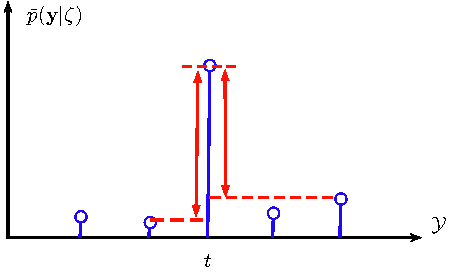
\includegraphics[width=0.48\textwidth]{./Figures/large_margin.pdf}\label{fig:small_entropy}} 
    \subfigure[]{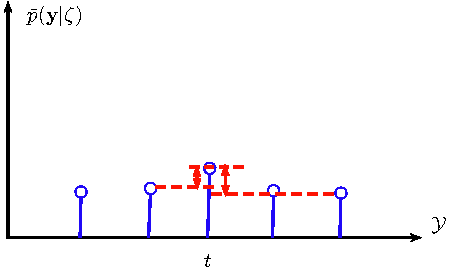
\includegraphics[width=0.48\textwidth]{./Figures/small_margin.pdf}\label{fig:large_entropy}}
    \caption{Two possible cases of $\bar{p}(\mathbf{y}|\zeta)$ when $\bar{\mathcal{L}}^{MAP}$ is minimized.  } 
    \label{fig:MAP_outputs}
\end{figure}


%----------------------------------------------------------------------------------------
%	SECTION 2
%----------------------------------------------------------------------------------------
\section{Training Undirected Graphical Models with Persistent Sequential Monte Carlo}
\label{sec:PSMC}
As analyzed in subsection \ref{subsec:MLE}, computing the exact likelihoods of CRFs for the maximum likelihood estimation (MLE) is in general intractable. 
Therefore, different approximations are used, \emph{e.g.} \emph{mean field} (MF), \emph{loopy 
belief propagation} (LBP) or \emph{pseudo likelihood} (PL) \citep{LBP, Kumar03,CRF,Accelerated_CRF}.  
In this section, general undirected graphicalmodels (UGMs) are considered, which include 
both Markov random fields (MRFs) and conditional random fields (CRFs). 
Without loss of generality, a UGM can be modeled as: 
\begin{eqnarray}
    p(\mathbf{x};\boldsymbol{\theta})&=&\frac{\exp\left(-E(\mathbf{x};\boldsymbol{\theta})\right)}{\mathbf{Z}(\boldsymbol{\theta})}
    \label{equ:MRF}\\
    \textit{Energy function:} & &\quad E(\mathbf{x};\boldsymbol{\theta})=-\boldsymbol{\theta}^\top \phi(\mathbf{x})
    \label{equ:energy}
\end{eqnarray}
with random variables $\mathbf{x}=[x_1,x_2,\dots,x_D]\in\mathcal{X}$, $\phi(\mathbf{x})$ is a $K$-dimensional vector of sufficient statistics, and parameter 
$\boldsymbol{\theta}\in \mathbb{R}^K$. $\mathbf{Z}(\boldsymbol{\theta})=\sum_{\mathbf{x}} \exp (\boldsymbol{\theta}^\top\phi(\mathbf{x}))$ is the partition function for global normalization. 
Note that $p(\mathbf{x};\boldsymbol{\theta})$ can be also a conditional probability although it is not explicitly written out. 
\begin{algorithm} [!t]                    
\caption{SAP for learning UGMs}          
\label{alg:SAP}                           
\begin{algorithmic}[1]
\REQUIRE ~~\ %Input
given a training data $\mathbf{x}^{(m)}$.  
\STATE  $t\gets 0$, initialize the proposal distribution $p(\mathbf{x};\boldsymbol{\theta}_0)$. 
\STATE  Randomly initialize $S$ sample particles $\{\bar{\mathbf{x}}_0^{(s)}\}_{s=1}^S$
\WHILE {! stop criterion}
\FOR {s=1:S}
\STATE evolve particle $\bar{\mathbf{x}}_t^{(s)}$ to $\bar{\mathbf{x}}_{t+1}^{(s)}$ with a transition operator which leaves $p(\mathbf{x};\boldsymbol{\theta}_t)$ invariant
\ENDFOR
\STATE Calculate the gradient:
\begin{equation*}
	\frac{\partial \tilde{\mathcal{L}}(\boldsymbol{\theta}|\mathcal{D})}{\partial \boldsymbol{\theta} }=\phi(\mathbf{x}^{(m)})-\frac{1}{S}\sum_{s=1}^S(\phi(\bar{\mathbf{x}}_t^{(s)}))
\end{equation*}
\STATE update $\boldsymbol{\theta}_{t+1}=\boldsymbol{\theta}_{t}+\eta_t \frac{\partial \tilde{\mathcal{L}}(\boldsymbol{\theta}|\mathcal{D})}{\partial \boldsymbol{\theta} }$
\STATE $t \gets t+1$, decrease learning rate $\eta_t$
\ENDWHILE
\ENSURE ~~\ %Output
estimated parameters  $\boldsymbol{\theta}^*=\boldsymbol{\theta}_t$  
\end{algorithmic}
\end{algorithm}



During the past decade, besides the approximation methods mentioned above, several sampling-based approximations were also developed for learning 
UGMs, \emph{e.g.} persistence contrastive divergence (PCD) \citep{tielemanPcd2008},  tempered transition (TT) \citep{Salakhutdinov_learningin} and parallel tempering (PT) \citep{desjardins2010}. 
All these learning methods for
UGMs can be considered as special cases of Robbins-Monro’s stochastic approximation procedure (SAP; \citealt{RobbinMonro,Younes1988}). A pseudo code of SAP for learning UGMs is provided in Algorithm \ref{alg:SAP}  
with different invariant transitions (\emph{e.g.} PCD is a SAP with Gibbs transitions). By linking SAP
and sequential Monte Carlo (SMC), PCD and other state-of-the-art learning algorithms can be cast into a
SMC-based interpretation framework. Moreover, within the SMC-based interpretation, two key factors
which affect the performance of learning algorithms are disclosed: \emph{learning rate} and \emph{high model complexity}.
Based on this rationale, the strengths and limitations of different learning algorithms can be analyzed
and understood in a new light.

Inspired by the understanding of learning UGMs from the SMC perspective, and the successes of global
tempering used in parallel tempering and tempered transition, a new learning algorithm, \emph{persistent sequential Monte Carlo} (PSMC) is put forward in this section to approach the
MLE in learning UGMs. The basic idea is to construct a long, persistent distribution sequence by 
inserting many tempered intermediary distributions between two successively updated
distributions. According to empirical results on learning several UGMs, the proposed PSMC out
performs other learning algorithms in challenging circumstances.

More technical details and results are presented in the paper II by the author. Furthermore, PSMC is also evaluated and compared against other relvelent learning algorithms 
on two practical tasks: \emph{image annotation} and \emph{image segmentation} in 
subsection \ref{subsec:graph_experiment}, where two conditional random fields are constructed and trained.    


\begin{shaded}
{\Huge II.} \textbf{Hanchen Xiong}, Sandor Szedmak, Justus Piater. {\it Towards Maximum Likelihood: Learning Undirected Graphical Models using Persistent Sequential Monte Carlo}, The 6th Asian Conference on Machine Learning (ACML2014), 
\end{shaded}
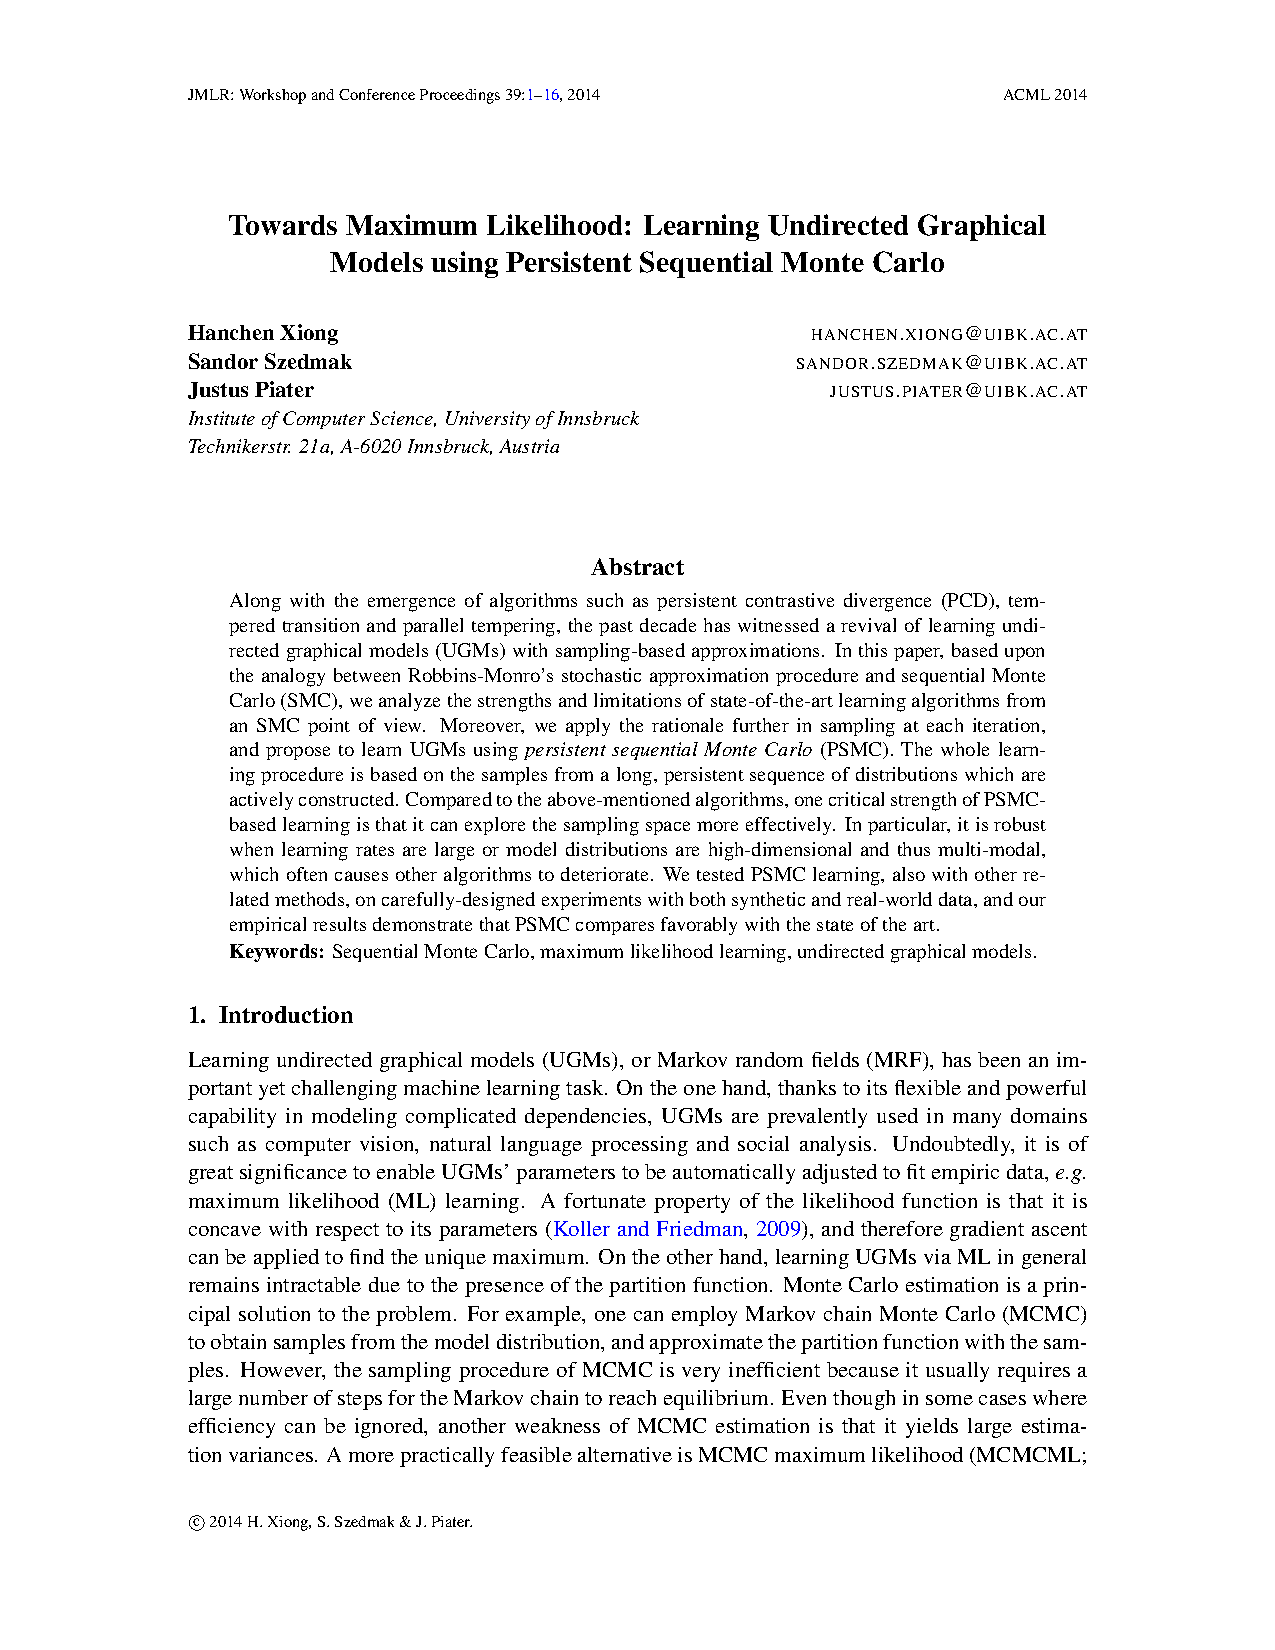
\includepdf[offset=3cm -2.5cm, scale=1, pages=-,pagecommand={\pagestyle{fancy}}]{./Papers/Xiong-2014-ACML.pdf}

\subsection {Training Conditional Random Fields for Image Annotation and Image Segmentation}
\label{subsec:graph_experiment}
In this subsection, some evaluations and comparison of different learning algorithms on two practical tasks, \emph{multi-label learning} and \emph{image 
segmentation}, are presented. Different from previous experiments in the paper II where generative models were learned, here discriminative models are used, \emph{i.e.}, two 
conditional random fields were employed. Generally speaking, let $\mathbf{x}$ denotes input and $\mathbf{y}\in \mathcal{Y}$ as output, the target is to 
learn an UGM:  
\begin{equation}
	p(\mathbf{y}|\mathbf{x})=\frac{\exp(\boldsymbol{\theta}^\top \phi(\mathbf{y},\mathbf{x}))}{\mathbf{Z}}
\end{equation}
where the partition function $\mathbf{Z}$ is
\begin{equation}
	\mathbf{Z}=\sum_{\mathbf{y}\in\mathcal{Y}}\exp(\boldsymbol{\theta}^\top \phi(\mathbf{y},\mathbf{x}))
\end{equation}
where $\phi(\mathbf{y},\mathbf{x})$ is defined based on task-oriented dependency structure. Note that the partition function $\mathbf{Z}$ is computed by 
marginalizing out only $\mathbf{y}$ because the interest here is a conditional distribution. Six algorithms 
were implemented: PCD-$H$, PCD-1, PT, TT, SMC and PSMC. Similar setups were used for all algorithms as in the paper II.  
Learning rate $\eta_t=\frac{1}{10+0.1*t}$ was used and 100 iterations were run. For each input $\mathbf{x}$, 
the size of particle set $\{ \hat{\mathbf{y}}^{(s)}\}$ is 200.  Similar to other supervised learning schemes, a regularization $\frac{1}{2}||\boldsymbol{\theta}||^2$ 
was added and a trade-off parameters was tunned via $k$ folder cross-validation ($k=4$).  

It is worth mentioning that better results can be expected in both experiments by running more iterations, using better learning rates or exploiting 
feature engineering. However, the purpose here is to compare different learning algorithms under the some conditional instead of defeat state-of-the-art 
results in multi-label learning study and image segmentation study respectively. Therefore, less effort was put in tunning algorithms and constructing 
sophisticated features. 

\subsubsection{Multi-Label Learning}
In multi-label learning, inter-label dependency is rather critical. Assume that input $\mathbf{x}\in \mathbb{R}^d$ and there are $L$ labels (\emph{i.e.} $\mathbf{y}\in\{-1,+1\}^L$), here all pairwise 
dependencies among $L$ labels were modeled, and therefore 
the constructed conditional random field is:
\begin{equation}
	p(\mathbf{y}|\mathbf{x})=\frac{\exp(\mathbf{y}^\top\mathbf{W}_E \mathbf{y}+\mathbf{y}^\top \mathbf{W}_v \mathbf{x})}{\mathbf{Z}}
	\label{equ:scene_model}
\end{equation}
where $\mathbf{W}_E\in \mathbb{R}^{L\times L}$ captures pairwise dependencies among $L$ labels (except diagonal entries) while $\mathbf{W}_v\in \mathbb{R}^{L\times d}$ reflects the 
dependencies between input $\mathbf{x}$ and all individual labels.   
In the test phase, with learned $\mathbf{W}_E$ and $\mathbf{W}_v$, for a test input $\mathbf{x}^\dagger$, the corresponding $\mathbf{y}^\dagger$ was predicted with 
100 rounds of gibbs sampling based on (\ref{equ:scene_model}).  

The \emph{scene} database \citep{scene_database} was used in the experiment.  In the database, scene images are associated with a few semantic labels.
There are 1121 training instances and 1196 test instances.  In total there are 6 labels ($L=6$) and a 294 dimensional feature were extracted from each image         
($\mathbf{x}\in\mathbb{R}^{294}$). Readers are referred to \cite{scene_database} for more details about the database and feature extraction.  

The performance of multi-label learning was evaluated using \emph{precision} (P), \emph{recall} (R), and the \emph{F1} measure (F). 
%For each label, the precision is 
%computed as the ratio of the number of images assigned the label correctly over the total number of images predicted to have the label, while the recall is the number of images 
%assigned the label correctly divided by the number of images that truly have the label. Then precision and recall are averaged across all labels. Finally, the F1 measure is calculated as 
%$F=2\frac{P\times R}{P+R}$.
The results of all six algorithms are presented in Table \ref{tab:scene_results}.     
The average number temperatures in PSMC is around 5, so PCD-5 was implemented. Also 5 temperatures were use in PT and TT.    
It can be seen that PSMC yields the best F1 measure 75.1, followed by PT and SMC with 74.6 and 73.4 respectively. The results of PCD-5 and TT             
are relative worse, while PCD-1 is the worst.  


\begin{table}
	\center
\begin{tabular}{cccc} 
\Xhline{2\arrayrulewidth} \\ 
       & Precision($\%$) & Recall($\%$) & F1($\%$) \\ \hline 
 PCD-1 & 57.7            & 59.3         & 58.5 \\
 PCD-5 & 70.3            & 72.6         & 71.4 \\
 TT    & 70.0            & 67.5         & 68.7 \\
 PT    & {\bf 72.2}      & 77.1         & 74.6 \\
SMC    & 71.7            & 75.1         & 73.4 \\
PSMC   & 71.9            & {\bf 78.5}   & {\bf 75.1} \\ 
\Xhline{2\arrayrulewidth}
 \end{tabular}
 \caption{A comparison of six learning algorithms on multi-label learning. }
	\label{tab:scene_results}
\end{table}

\subsubsection{Image Segmentation} 
Image segmentation is  essentially a task to predict the semantic label of all image pixels or blocks.    
Inter-label dependences within neighbourhood are usually exploited in image segmentation. For instance, by dividing an image into equal size and non-overlapping 
blocks, the label of a block does not only depend on the appearance of the block, but also the labels of its neighbouring blocks. For simplicity, here 
only binary labels are considered (\emph{e.g.} foreground and background). 
In addition, blocks and inter-label dependencies are assumed to be position-irrelevant. Therefore, a conditional random filed can 
be constructed as:               
\begin{equation}
	p(\mathbf{y}|\mathbf{x})=\frac{\exp(\sum_{u,v\in E}y_u W_e y_v+\sum_{v\in V} y_v \mathbf{w}_v^\top \mathbf{x}_v) }{\mathbf{Z}}
\end{equation}
where $y_v\in\{-1,+1\}$, $E$ denotes the set of all edges connecting neighbouring blocks, $W_e\in\mathbb{R}$ encodes the dependency between neighbouring labels, $V$ denotes the set of all 
block's labels and $\mathbf{w}_v\in \mathbb{R}^{d\times 1}$ encodes the dependency between a block's label and its appearance which is represented by a $d$-dimensional feature $\mathbf{x}_v\in\mathbb{R}^d$.    
Similar to the multi-label experiment, desired labels are predicted via 100 round gibbs sampling in test phase.      

The binary segmentation database from \cite{img_seg_database} was used.  Each image is divided into non-overlapping blocks of 
size $16\times16$ and each block is annotated with either ``man-made structure" (MS) or ``nature structure" (NS). 
Overall, there are 108 training images and 129 test images. The training set contains 3004 MS blocks and 36269 NS blocks, while the test set 
contains 6372 MS blocks and 43164 NS blocks.
For each block, its appearance is 
represented by a 3-dimensional features which includes the mean of gradient magnitude, the 'spikeness' of the count-weighted histogram of gradient orientations, 
the angle between the most frequent orientation and the second most frequent orientation. The feature was designed to fit this specific application.        
More explanation of the database and feature design can be found in \cite{img_seg_database}. 


It is found that the average number of temperatures in PSMC is 20, therefore PCD-20 was run and 20 temperatures were used in TT and PT. The segmentation performance of 
six algorithms are quantified with confusion matrices, which are presented in Figure \ref{fig:img_seg_results}. It can be seen that PSMC outperforms all others (by checking the diagonal 
entries of confusion matrices).      
For qualitative comparison, an example image and corresponding segmentations are shown in Figure \ref{fig:img_seg_example}.  It can be seen that the segmentation by PSMC is closer to the ground truth 
compared to others. 
\begin{figure}[t!] 
    \centering
    \subfigure{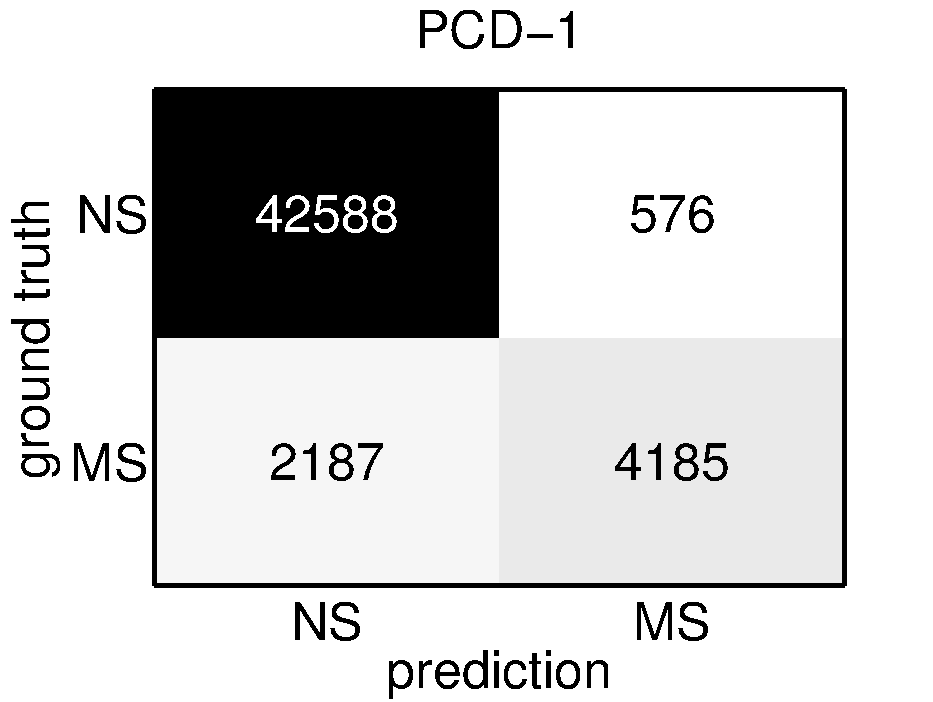
\includegraphics[width=0.48\textwidth]{./Figures/CM_PCD_1}\label{fig:CM_PCD_1}}
    \subfigure{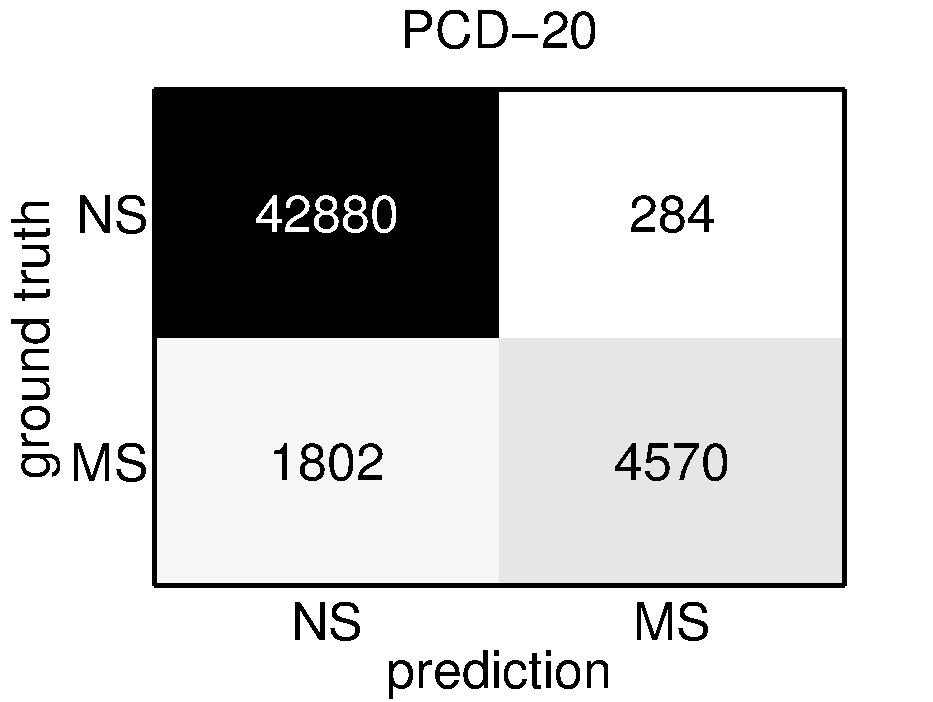
\includegraphics[width=0.48\textwidth]{./Figures/CM_PCD_20}\label{fig:CM_PCD_20}}
	\subfigure{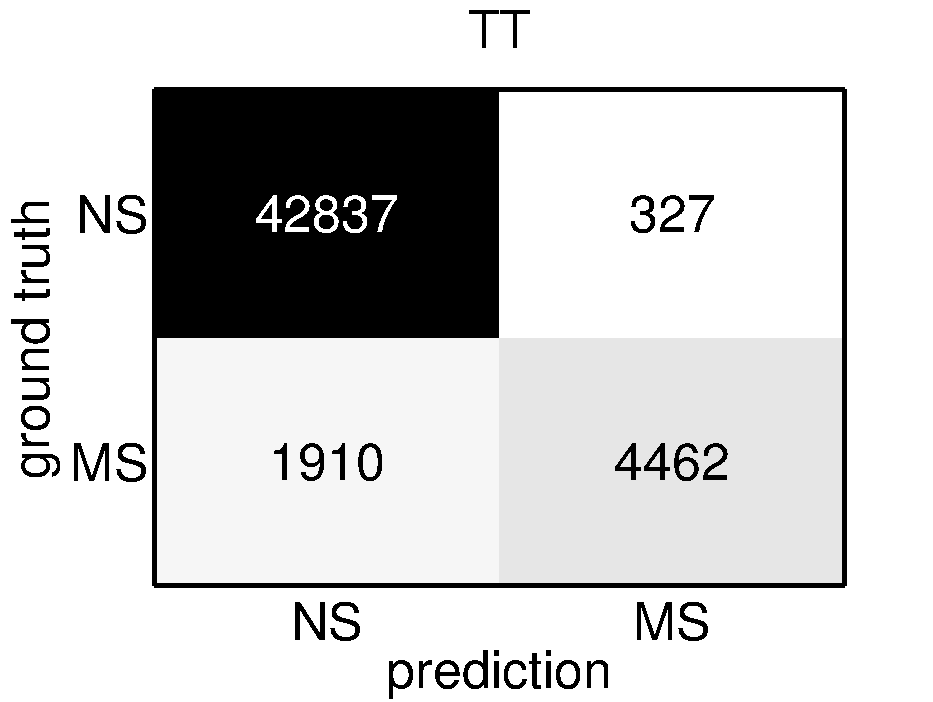
\includegraphics[width=0.48\textwidth]{./Figures/CM_TT}\label{fig:CM_TT}}
	\subfigure{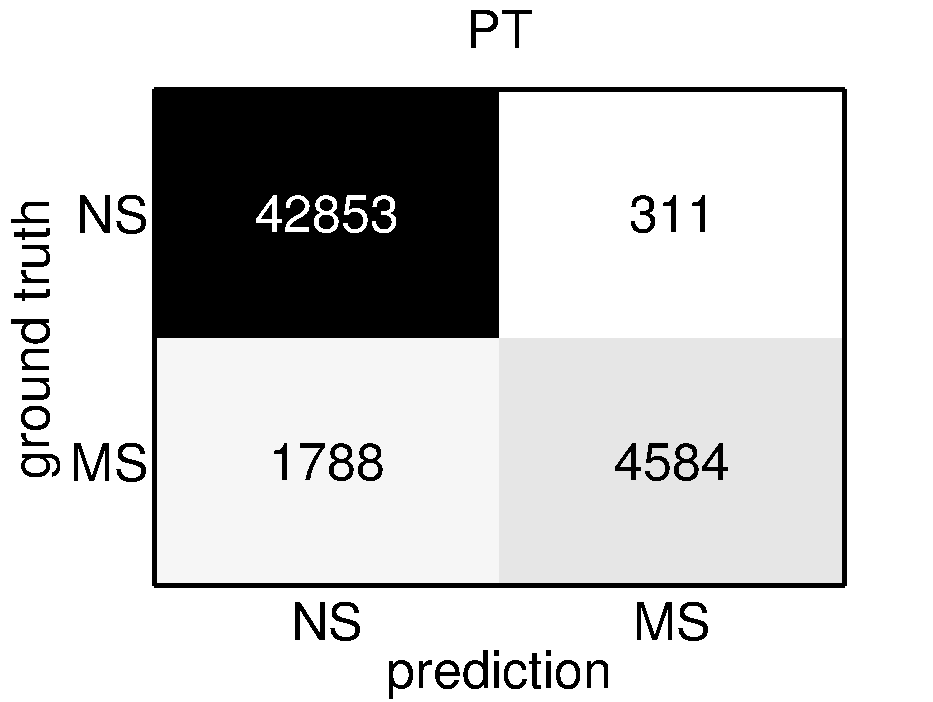
\includegraphics[width=0.48\textwidth]{./Figures/CM_PT}\label{fig:CM_PT}}
	\subfigure{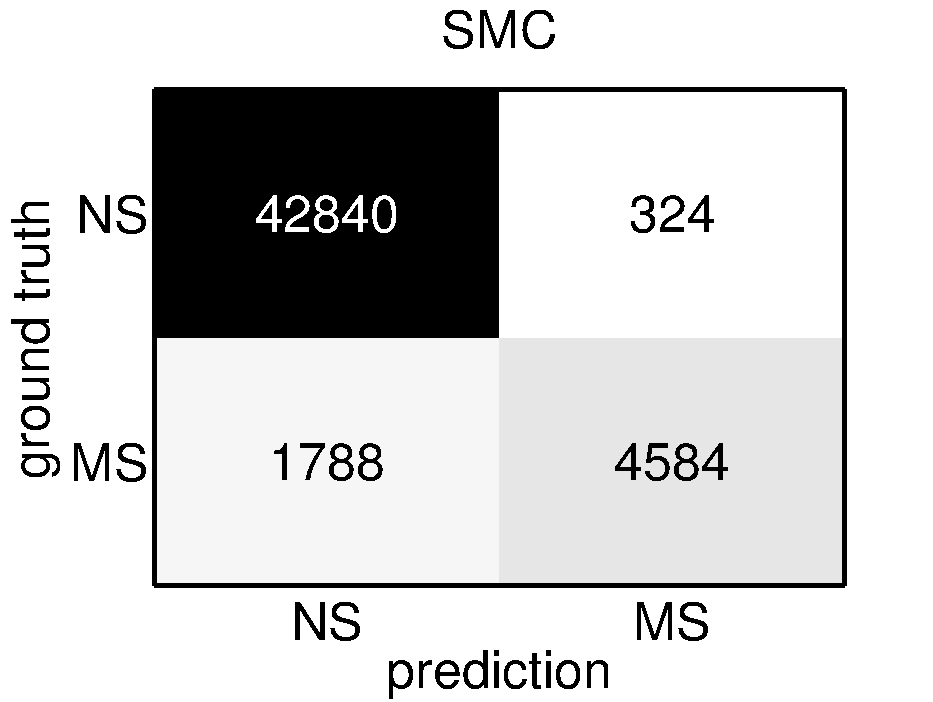
\includegraphics[width=0.48\textwidth]{./Figures/CM_SMC}\label{fig:CM_SMC}}
	\subfigure{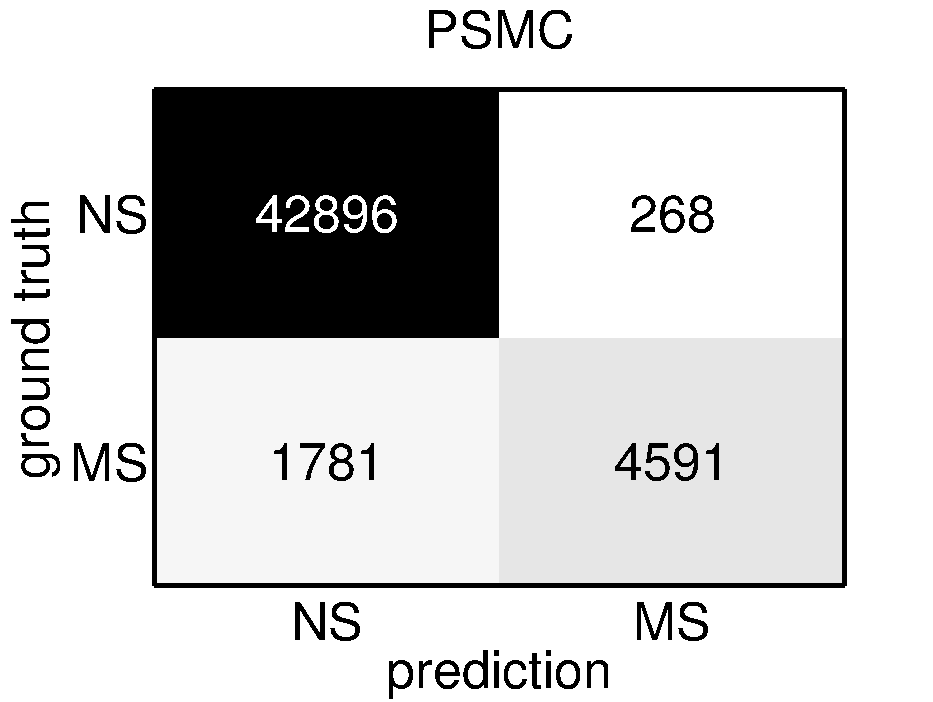
\includegraphics[width=0.48\textwidth]{./Figures/CM_PSMC}\label{fig:CM_PSCM}}
    \caption{Confusion matrices of binary segmentation by six algorithms.}   
    \label{fig:img_seg_results}
\end{figure}

\begin{figure}[t!] 
    \centering
    \subfigure[]{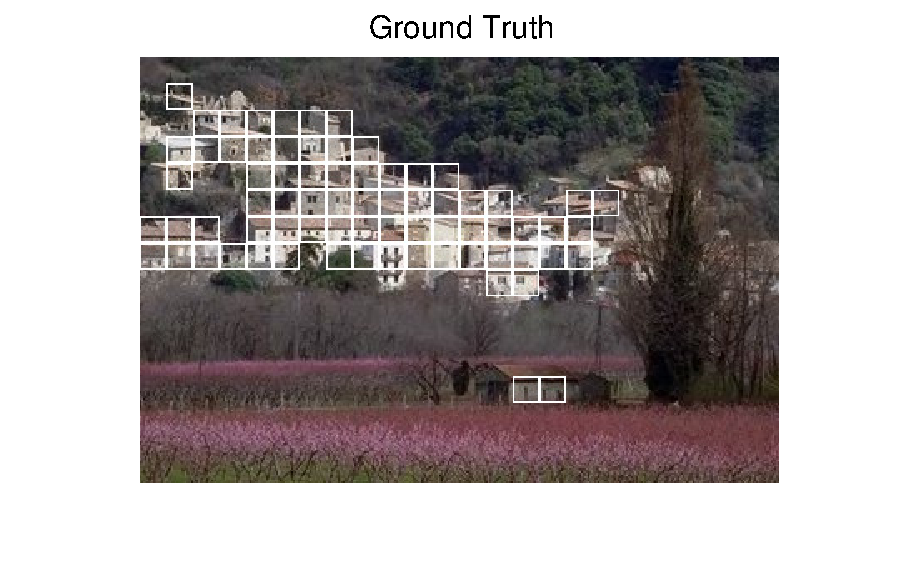
\includegraphics[width=0.7\textwidth]{./Figures/img_seg_GT}\label{fig:img_seg_GT}} \\
    \subfigure[]{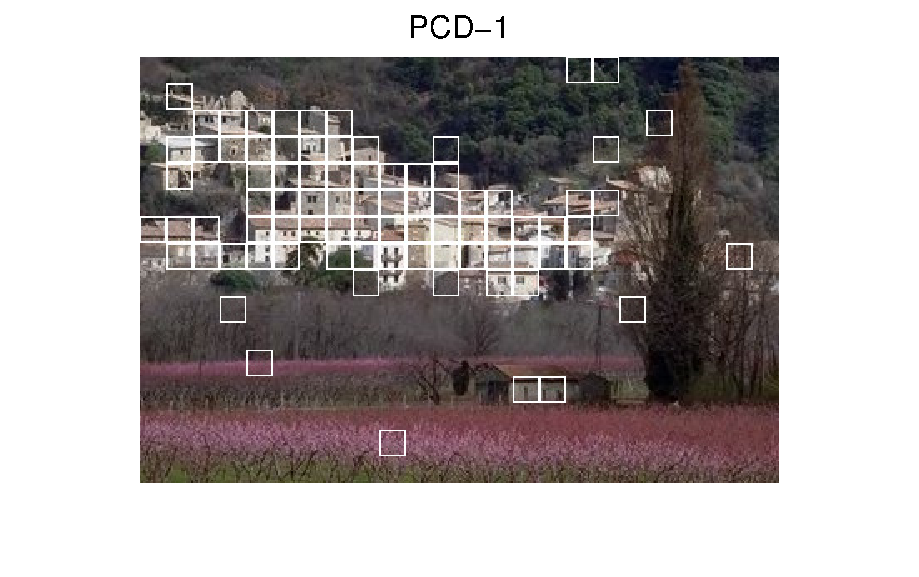
\includegraphics[width=0.49\textwidth]{./Figures/img_seg_PCD_1}\label{fig:img_seg_PCD_1}}
    \subfigure[]{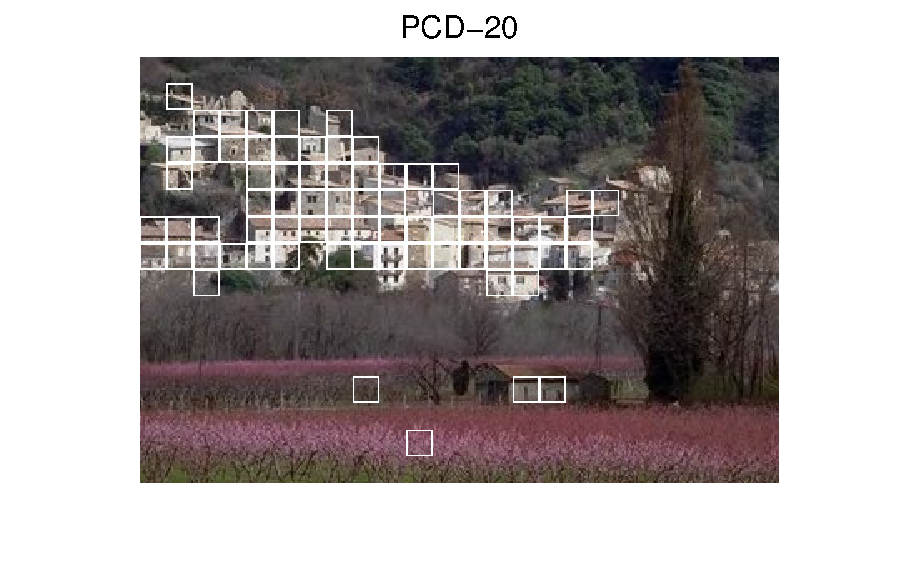
\includegraphics[width=0.49\textwidth]{./Figures/img_seg_PCD_20}\label{fig:img_seg_PCD_20}}
	\subfigure[]{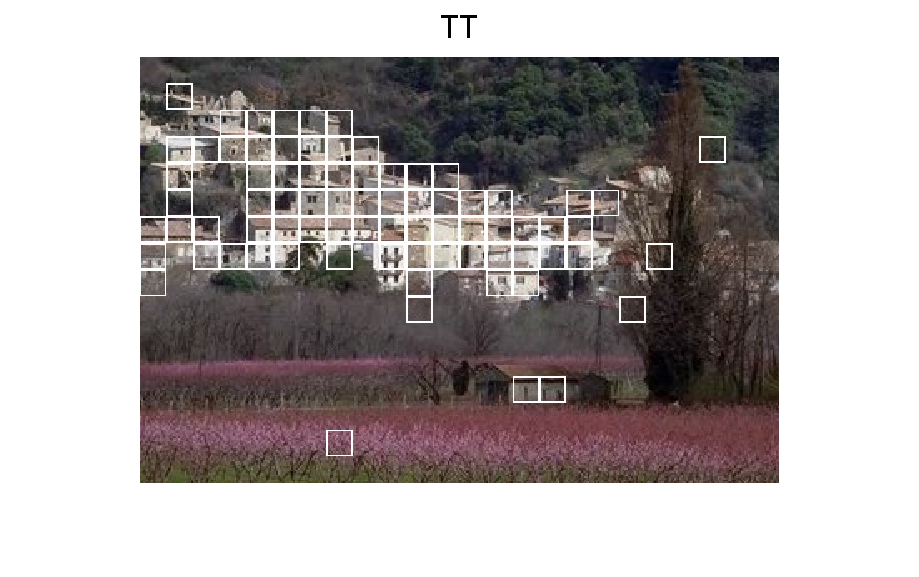
\includegraphics[width=0.49\textwidth]{./Figures/img_seg_TT}\label{fig:img_seg_TT}}
	\subfigure[]{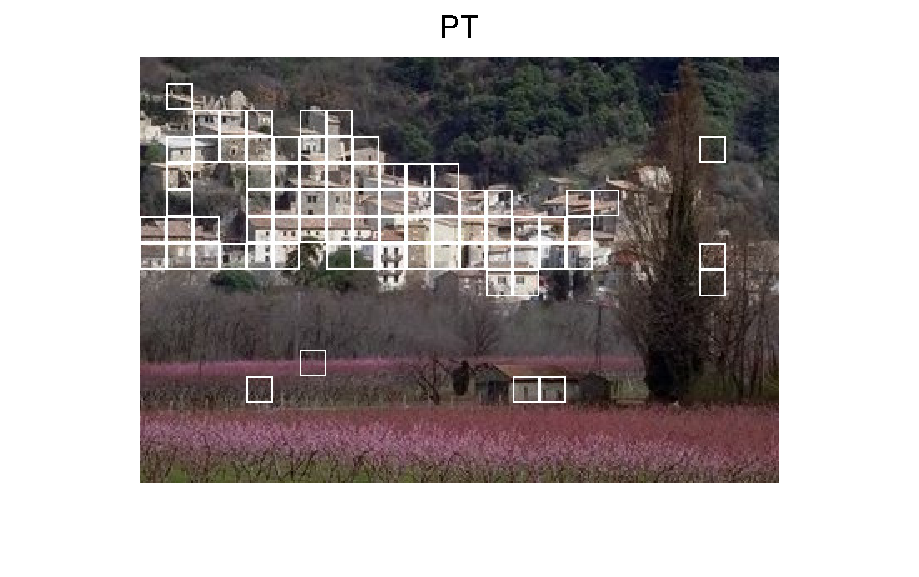
\includegraphics[width=0.49\textwidth]{./Figures/img_seg_PT}\label{fig:img_seg_PT}}
	\subfigure[]{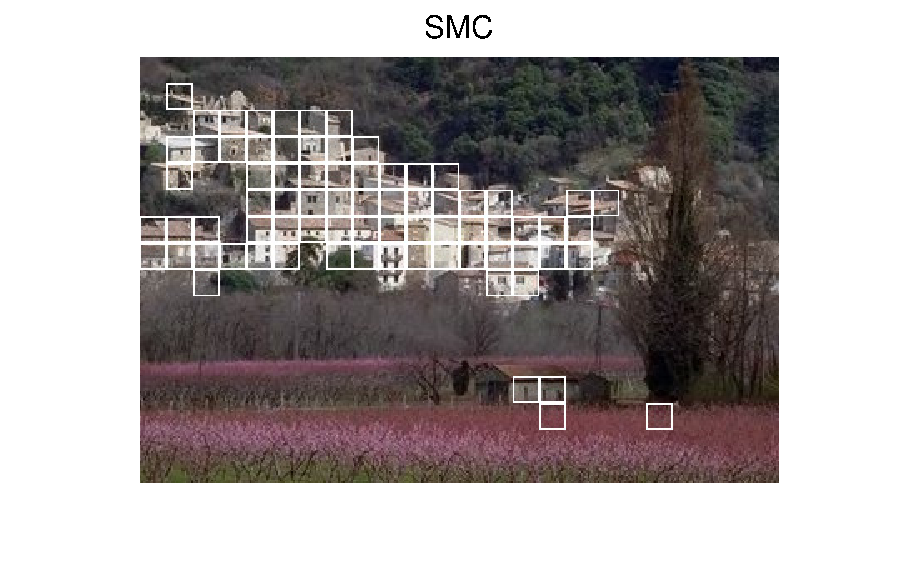
\includegraphics[width=0.49\textwidth]{./Figures/img_seg_SMC}\label{fig:img_seg_SMC}}
	\subfigure[]{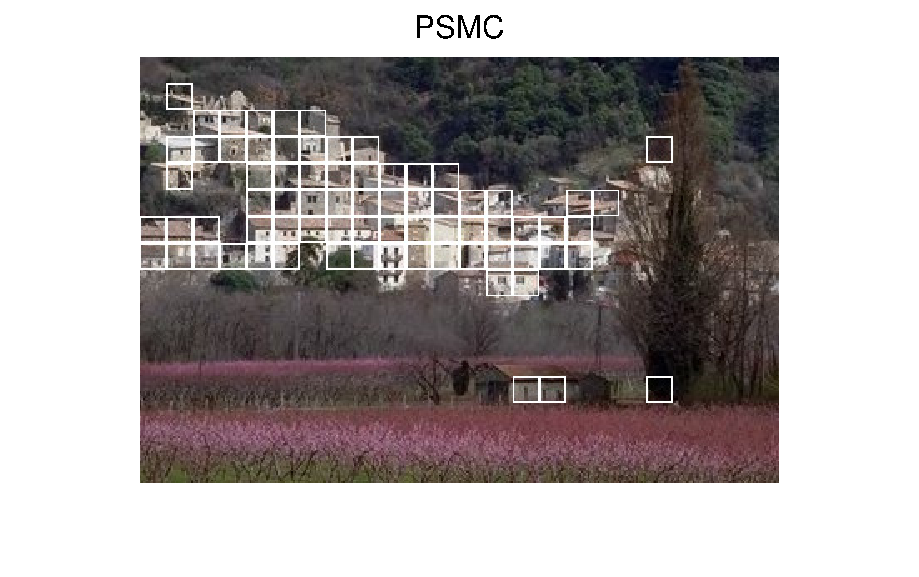
\includegraphics[width=0.49\textwidth]{./Figures/img_seg_PSMC}\label{fig:img_seg_PSCM}}
    \caption{An example image and corresponding segmentations by six algorithms. Regions within white boxes are predicted as ``man-made structure'' while 
	the remaining are ``nature structure''. }   
    \label{fig:img_seg_example}
\end{figure}


